\documentclass[a4paper,12pt]{article}
\usepackage[a4paper,top=1.3cm,bottom=2cm,left=1.5cm,right=1.5cm,marginparwidth=0.75cm]{geometry}
%%% Работа с русским языком
\usepackage{cmap}					% поиск в PDF
\usepackage{mathtext} 				% русские буквы в фомулах
\usepackage[T2A]{fontenc}			% кодировка
\usepackage[utf8]{inputenc}			% кодировка исходного текста
\usepackage[english,russian]{babel}	% локализация и переносы

\usepackage{graphicx}
\usepackage{mathtools}
\usepackage{wrapfig}
\usepackage{tabularx}
\usepackage{amssymb}
\usepackage{hyperref}
\usepackage[rgb]{xcolor}
\hypersetup{colorlinks=true,urlcolor=blue}
\setcounter{secnumdepth}{0}
%% Шрифты
\usepackage{euscript}	 % Шрифт Евклид
\usepackage{amsmath}
\usepackage{mathtools}
%%% Заголовок
\author{Tsvetkova Amelia}
\title{Лабораторная работа по общей физике}

\date{\today}
\begin{document}
\begin{titlepage}
    \newpage
    \begin{center}
    {\large МОСКОВСКИЙ ФИЗИКО-ТЕХНИЧЕСКИЙ ИНСТИТУТ (НАЦИОНАЛЬНЫЙ ИССЛЕДОВАТЕЛЬСКИЙ УНИВЕРСИТЕТ)}
    \vspace{1cm}

    {\largeФизтех-школа аэрокосмических технологий}
    \vspace{6em}
    \end{center}
    
    \vspace{1.2em}

    \begin{center}
    \Large Лабораторная работа №4.5.1 \\
    Гелий-неоновый лазер
    \linebreak
    \end{center}
    
    \vspace{11em}
    
    \begin{flushright}
                       {\large Работу выполнила\\
                       Цветкова Амелия Антоновна\\
                       Б03-303 }
    \end{flushright}

    \vspace{\fill}

    \begin{center}
    Долгопрудный, 2025
    \end{center}

    \end{titlepage}

\paragraph{Цель работы:} Изучение основных принципов работы гелий-неонового лазера, свойств лазерного излучения и измерение усиления лазерной трубки.

\paragraph{В работе используются:} объект исследования - активный элемент от гелий-неонового лазера ЛГ-75 с блоком питания, дополнительный He-Ne-лазер для юстировки и измерений, модулятор излучения (обтюратор), фотодиоды, зерркала, поляроид, компьютер со звуковой картой.

\section{Теоретические сведения}
\subsection{Общие принципы работы лазера}

\texttt{Лазер}, или \texttt{оптический квантовый генератор}, - источник квазимонохроматического и узконаправленного высококогерентного потока излучения, работающий за счет квантово-механического эффекта вынужденного излучения.

Главными элементами лазера являются \texttt{оптический} \texttt{резонатор} и расположенная в нем \texttt{активная} \texttt{среда}, способная усиливать проходящее через нее излучение.

Резонатор обеспечивает создание положительной обратной связи в лазере и превращает его в генератор излучения. Также в резонаторе происходит накопление энергии излучения и отбор узких резонансных линий из спектра излучения, рождающегося в среде. Одно из зеркал резонатора обычно имеет несколько меньший коэффициент отражения, что позволяет выпускать через него часть излучения в виде узконаправленного высокомонохроматического пучка.

Принцип усиления в активной среде основан на использование эффекта \texttt{вынужденного} (индуцированного) излучения. Вынужденное излучение - процесс, обратный поглощению фотона атомом. В нем атом, находящийся в возбужденном состоянии, под действием налетающего на него фотона переходит в состояние с меньшей энергией, испуская при этом еще один фотон, частота, поляризация и фаза которого совпадают с таковыми у исходного фотона. Другими словами, падающий и рожденный в результате индуцированного излучения фотоны являются полностью когерентными.

\begin{figure}[h]
\centering
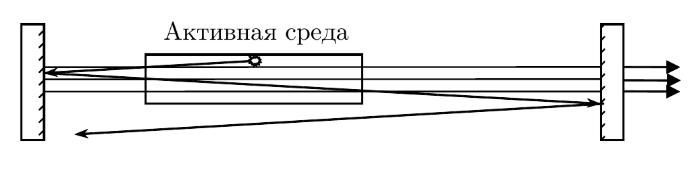
\includegraphics[width=0.5\linewidth]{img4.png}
\caption{Схема лазера}
\label{img4}
\end{figure}

Вероятность поглощения фотона при взаимодействии с атомом в невозбужденном состоянии равна вероятности индуцированного испускания при взаимодействии фотона с возбужденным атомом. Поэтому для того, чтобы среда в целом усиливала излучение, количество возбужденных атомов должно быть больше, чем количество невозбужденных. Такое состояние среды не является термодинамически равновесным и наз. состоянием с \texttt{инверсной заселенностью} уровней. Для создания инверсной заселенности используют различные методы \texttt{накачки}. Источником первичных фотонов служит процесс \texttt{спонтанного} излучения возбужденных атомов.

\subsubsection{Элементарные процессы}

Энергия электронов в атомах способна принимать лишь некоторый дискретный набор значений - энергетических уровней $E_i$. Если энергия электронов атома минимальна (и равна $E_0$), то говорят, что атом находится в \textit{основном состоянии}. Если атом находится на любом другом энергетическом уровне $E_i > E_0$, то говорят, что атом находится в \textit{возбужденном} состоянии. 

Изменение энергии электрона в атоме может сопровождаться испусканием или поглощением энергии в виде кванта электромагнитного излучения - фотона. Энергия фотона равна $\hbar w$, где $w$ - частота колебаний электромагнитного поля, $\hbar = h/2\pi (h\approx 6.6\cdot10^{-34}\text{Дж}\cdot\text{с} - \text{постоянная Планка})$. Электрон в атоме, находящийся в состоянии $E_0$ или $E_1$, может провзаимодействовать с фотоном энергии $\hbar w$, если выполняется равенство $E_1-E_0=\hbar w$.

\begin{figure}[h]
\centering
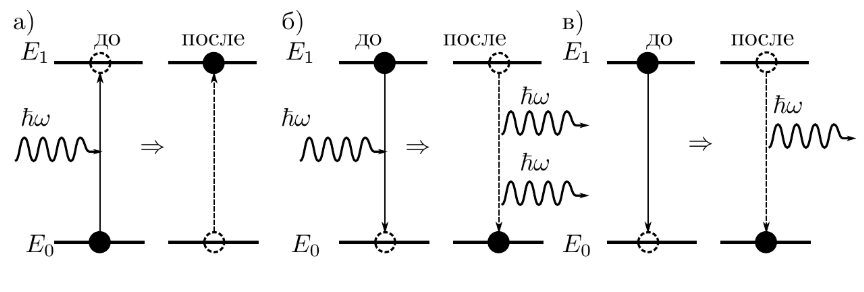
\includegraphics[width=0.6\linewidth]{img5.png}
\caption{Переходы между уровнями $E_1$ и $E_0$}
\label{img5}
\end{figure}

Три главных элементарных процесса, определяющих взаимодействие излучения с активной средой лазера:
\begin{enumerate}
    \item Поглощение фотона невозбужденным атомом $\hbar w + A \rightarrow A^*$. Атом при взаимодействии с внешним электромагнитным полем поглощает квант энергии $\hbar w$ и переходит из состояния $E_0$ в состояние $E_1=E_0+\hbar w$
    \item Вынужденное излучение при взаимодействии атома с падающим на него электромагнитным полем $\hbar w + A^* \rightarrow A+2\hbar w$. При этом взаимодействии атом переходит в основное состояние, испуская еще один фотон той же частоты $w$.

    Вероятности того, что атом поглотит или вынужденно испустит фотон, отличны от нуля только для поля резонансной частоты $\hbar w = E_1-E_0$. Кроме того вероятности переходов равны между собой и пропорциональны спектральной плотности энергии внешнего поля $\rho_w$.
    \begin{equation}
        W_{0\rightarrow 1} = W_{1\rightarrow 0} = B\rho_w,
    \end{equation}
    где $W$ - вероятности для соотвествующих переходов, $B$ - коэффициент, характеризующий переходы между рассматриваемыми уровнями энергии, не зависящий от величины поля (наз. \texttt{коэффициент Эйнштейна} для вынужденных переходов)
    \item Спонтанное излучение возбужденным атомом $A^* \rightarrow A +\hbar w$. Время жизни возбужденных состояний - конечная величина, поэтому по прошествии некоторого времени возбужденный атом испустит фотон частоты $w=(E_1-E_0)/\hbar$. Скорость этого процесса является константой, не зависящей от наличия внешнего поля. Фаза и направление расспространения испущенного фотона будут случайны, так что данный процесс препятствует сохранению когерентности излучения лазера.
\end{enumerate}

\subsubsection{Коэффициент усиления}

Изменение интенсивности электромагнитной волны $dI$, прошедшей участок поглощающей среды толщиной $dx$, пропорционально интенсивности волны на этом участке $I(x): dI=-\alpha Idx$, где $\alpha$ - \texttt{коэффициент поглощения} на единицу длины среды. Если $\alpha=const$, то в результате интегрирования получаем, что интенсивность волны в среде изменяется по закону
$$
I(x) = I_0(x)\exp(\alpha x)
$$
(\texttt{закон Бугера-Ламберта-Бера}). Если $\alpha <0$, то говорят о \texttt{коэффициенте усиления} среды $\gamma=-\alpha$, интенсивность при этом экспоненциально нарастает:
\begin{equation}
    I(x) = I_0\exp(\gamma x)
\end{equation}

Рассмотрим прохождение через среду плоской электромагнитной волны, частота $w$ которой удовлетворяет резонансному условию $\hbar w=E_1-E_0$, где $E_1$ и $E_0$ - некоторые уровни энергии атомов среды.

Пусть $N_1$ и $N_0$ - концентрации атомов с энергиями $E_1$ и $E_0$ соответственно. Доля невозбужденных атомов, поглощающих квант излучения в единицу времени, равна:
$$
\frac{dN_0}{N_0}=W_{0\rightarrow1}dt=B\rho_w dt
$$
Убыль фотонов в единице объема при этом равна
$$
dN_\text{Ф}^- = -dN_0 = -B\rho_w dt
$$
Аналогично, количество фотонов $dN_\text{Ф}^+$, рожденных за счет вынужденного излучения, равно
$$
dN_\text{Ф}^+=B\rho_w N_1 dt
$$

При прохождении волны сквозь среду изменение интенсивности волны пропорционально суммарному количеству рожденных и поглощенных квантов. Тогда для волны, прошедшей участок длиной $dx$ за время $dt=dx/v$, где $v=c/n$ - скорость волны, относительное изменение интенсивности равно
$$
\frac{dI}{I} = \frac{dN_\text{Ф}^+ + dN_\text{Ф}^-}{\rho_w/\hbar w} = B\frac{\hbar w}{v}(N_1-N_0)dx
$$
Таким образом, коэффициент усиления волны с частотой $w$ в активной среде лазера равен 
\begin{equation}
    \gamma = B\frac{\hbar w}{v}\Delta N ,
\end{equation}
где $\Delta N=N_1-N_0$. Отсюда видно, что \textit{среда является усиливающей} ($\gamma>0$), если концентрация атомов на верхнем уровне больше, чем на нижнем: $N_1>N_0$.

\subsubsection{Спектр генерации. Доплеровское уширение}

В реальности линия поглощения/излучения имеет конечную ширину $\Delta w_\gamma$, и коэффициент усиления должен быть домножен на функцию, пропорциональную форме контура этой спектральной линии. То есть коэффициент усиления $\gamma(w)$ есть функция частоты с острым максимумом вблизи резонансной частоты $w=(E_1-E_0)/\hbar$, обладающая некоторой конечной шириной $\Delta w_\gamma$.

Ширина спектра усиления активной среды лазера $\Delta w_\gamma$ (\texttt{спектра генерации}) определяется \textit{устественной шириной} резонансной линии лазерного перехода и различными \textit{механизмами уширения}.

\begin{figure}[h]
\centering
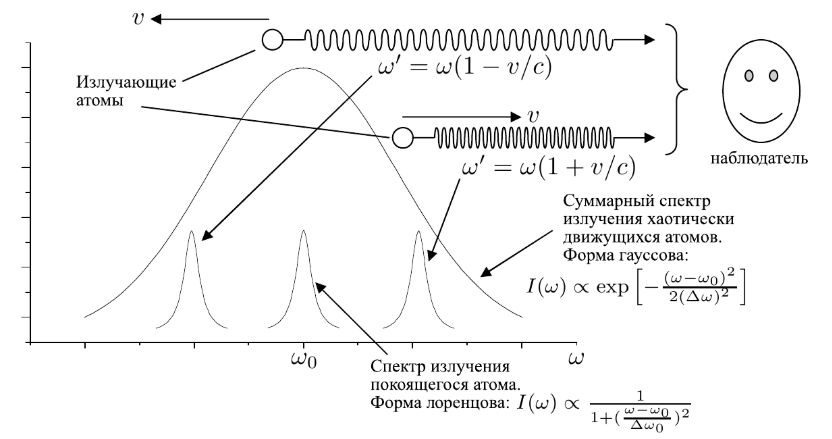
\includegraphics[width=0.5\linewidth]{img6.png}
\caption{Доплеровское уширение спектра излучения атомов вследствие теплового движения}
\label{img6}
\end{figure}

Естественная ширина линии - внутренняя характеристика атома, определяемая строением его энергетических уровней. Если известно время жизни возбужденного состояния $\tau_e$, естественная ширина $\Delta w_e \sim 2\pi/\tau_e$. В модели цугов время $\tau_e$ можеть быть отождествлено с длительностью цуга, излучаемого отдельным атомом.

Основным механизмом уширения в газовых лазерах, определяющим ширину спектральной линии излучения среды, явдяется \textit{эффект Доплера}, действие которого схематически изображено на рис.$\ref{img6}$.

В лазерной трубке атомы среды учааствуют в хаотическом тепловом движении. Частота излучения движущегося источника сдвинута относительно неподвижного источника; в нерелятивистском случае
$$
\frac{\Delta w_\text{Д}}{w}\sim \frac{v}{c}\cos{\alpha}
$$
где $\alpha$ - угол между вектором скорости и направлением на наблюдателя. Результирующий спектр излучения есть сумма вкладов от большого количества атомов среды. Поскольку при хаотическом движении $\cos{\alpha}$ принимает значения от 1 до -1, то полуширина линии приблизительно составляет
\begin{equation}
    \Delta w_\text{Д}\sim w\frac{v_T}{c} = \frac{w}{c}\sqrt{\frac{8k_\text{Б}T}{\pi m}}
\end{equation}
где $v_T$ - средняя тепловая скорость движения атомов.

\subsubsection{Условие достижения порога генерации}

Предположим, что активная среда с коэффициентом усиления $\gamma$ находится между двумя зеркалами с коэффициентами отражения по энергии $r_1$ и $r_2$. Пусть световой пучок распространяется из некоторой точки внутри резонатора и после отражения от двух зеркал возвращается в эту же точку. При длине промежутка $L$ \texttt{усиление} за один полный проход резонатора равно
$$
G=e^{2\gamma L}
$$

Учтем, что в лазере имеются дополнительные потери энергии, так что за один проход интенсивность из-за них составит долю T от исходной. Для самовозбуждения лазера необходимо, чтобы усиление было достаточным для компенсации всех потерь при полном обходе резонатора: $r_1r_2TG\geq 1$, откуда
\begin{equation}
    e^{\gamma L}\geq \frac{1}{\sqrt{Tr_1r_2}}
\end{equation}
или
$$
2\gamma L \geq -\ln{T} - \ln{r_1r_2}
$$

Заметим, что коэффициент усиления $\gamma(w)$ зависит от частоты и генерация может просисходить в диапазоне частот $w\pm\Delta w_\text{Г}$.

В лазерах с непрерывной генерацией в установившемся режиме потери излучения в точности компенсируются усилением, то есть усиление активного элемента за один проход равно $G=1/(Tr_1r_2)$. Чтобы лазер имел ненулевую мощность выходного ищлучения, активный элемент лазера должен иметь запас по усиелнию, то есть при отключении положительной обратной связи усиление должно превышать порог. При подключении обратной связи и выходе на стационарный режим генерации усиление автоматически падает до величины $1/(Tr_1r_2)$ за счет сброса возбужденных атомов с верхнего лазерного уровня на нижний лазерным излучением.

\begin{figure}[h]
\centering
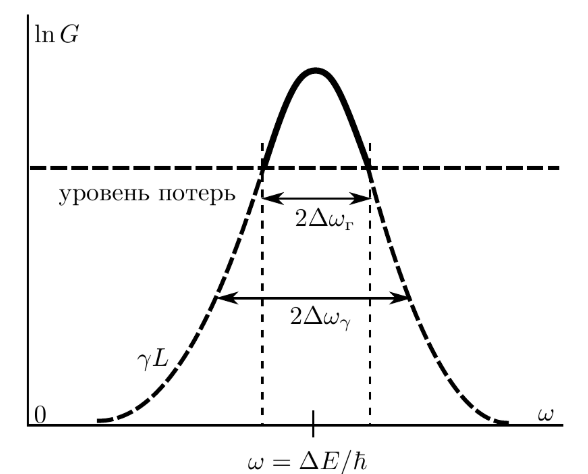
\includegraphics[width=0.5\linewidth]{img7.png}
\caption{Контур усиления и уровень потерь}
\label{img7}
\end{figure}

\subsubsection{Инверсная заселенность. Накачка}

Для создания среды, которая способна усиливать проходящее через нее излучение, необходимо, чтобы концентрация атомов на верхнем лазерном уровне была больше, чем на нижнем: $N_1>N_0$. В таком случае говорят, что уровни энергий атомов в активной среде имеют \texttt{инверсную заселенность}.

Система в состоянии инверсной заселенности, приведенная в контакт с окружающей средой, быстро отдаст ей избыток энергии и вернется к нормальной заселенности. Однако если имеется постоянная подкачка энергии извне, то неравновесное состояние может быть \textit{стационарным}.

Для создания инверсной заселенности уровней используют различные методы \texttt{накачки}: атомы "перекачиваются" из основного состояния в возбужденного с помощью внешних источников энергии. В качестве таких источников часто используются источники электромагнитного излучения нужной частоты (\texttt{оптическая накачка}). 

Ввиду того, что вероятность поглощения равна вероятности вынужденного испускания, \textit{инверсную заселенность в двухуровневой системе невозможно создать оптической накачкой}. Поэтому для создания инверсной населенности используют трех- и четырехуровневые системы.

\begin{figure}[h]
\centering
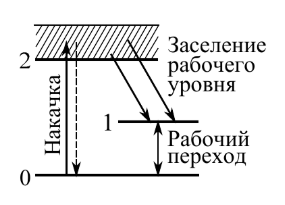
\includegraphics[width=0.2\linewidth]{img8.png}
\caption{Схема получения инверсной заселенности в трехуровневой системе}
\label{img8}
\end{figure}

Излучение накачки переводит атомы из состояния 0 в состояние 2. Из состояния 2 атомы могут вернуться либо в состояние 0, либо перейти в 1. На уровне 1 атомы будут накапливаться в том случае, если время жизни на нем велико. При этом условии на этом уровне можно накопить достаточное количество атомов, превосходящее числом количество атомов в основном состоянии. Время жизни $\tau$ связано с шириной уровня соотношением неопределенностей $\Delta E\tau\sim\hbar$, поэтому желательно, чтобы уровень 1 был узким. Уровень 2 должен быть широким - в этом случае удается полезно использовать заметную часть спектра оптического излучения накачки. Чаще всего роль уровня 2 играет широкая полоса. Переход $2\rightarrow 1$ нередко является безызлучательным; в таких переходах излишняя энергия атома передается не кванту излучения, а кристаллической решетке или сталкивающимся атомам.

\subsection{Модовый состав лазерного излучения}

\texttt{Модами} наз. стационарные типы колебаний электромагнитного поля в резонаторе, различающиеся частотой и пространственным распределением амлитуды поля.

\subsubsection{Продольные моды}

Зеркала обеспечивают возможность многократного прохода плоской волны, если ее волновой вектор направлен \textit{по оси} интерферометра $\vec{k}=(0,0,k)$. Если же он имеет наклон к оси, то после нескольких проходов волна покинет область пространства между зеркалами и не будет в достаточной мере усилена.

\subsection{Гелий-неоновый лазер}

Рассмотрим механизм возникновения усиелния в рабочей среде гелий-неонового лазера. Лазерная трубка заполняется смесью гелия и неона в соотношении от 5:1 до 10:1 с общим давлением порядка 100 Па, при котором легко возбудить постоянный электрический разряд. Рабочее лазерное вещество - неон. Гелий используется для избирательного заселения верхнего рабочего уровня неона. Атомы гелия возбуждаются при столкновении с разогнанными в электрическом поле разряда электронами. Передача энергии от возбужденных атомов гелия к атомам неона осуществляется при столкновениях между ними. Известно, что наиболее эффективно передача энергии от атома к атому происходит в резонансном случае. 

\begin{figure}[h]
\centering
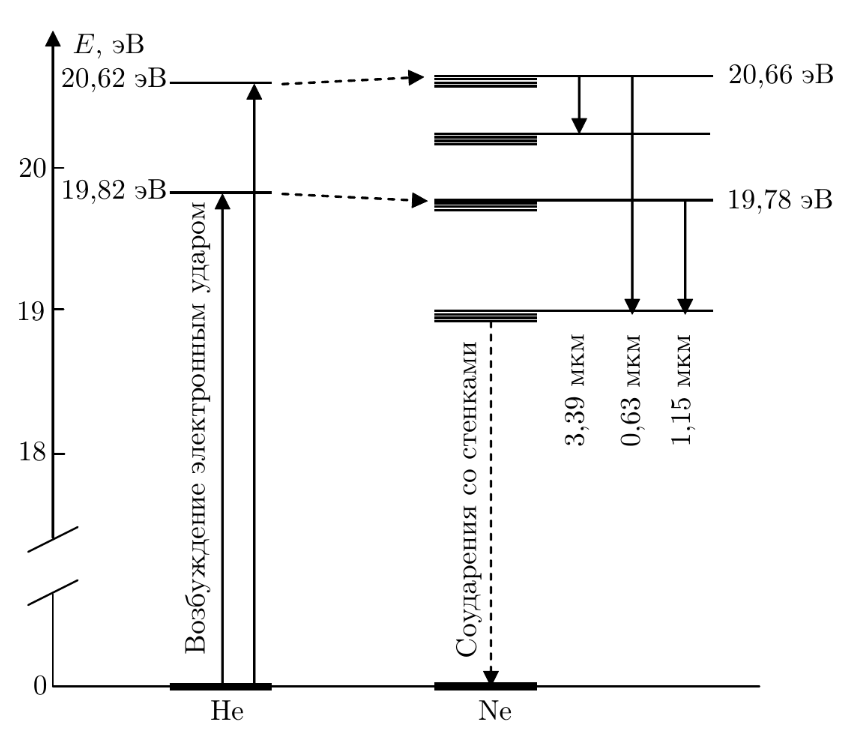
\includegraphics[width=0.6\linewidth]{img1.png}
\caption{Энергетическая схема работы гелий-неонового лазеры}
\label{img1}
\end{figure}

Упрощенная схема энергетических уровней атомов гелия и неона изображена на рис.$\ref{img1}$. Из него видно, что энергии двух уровней атома гелия действительно близки к двум уровням неона, что приводит к эффективной передаче энергии от гелия к неону. Генерация лазерного излучения атомами неона получена в лабораторных условиях на более чем 200 переходах. Однако во всех промышленных лазерах на неоне для увеличения эффективности накачки используют селективное заселение верхних лазерных уровней атомами гелия, поэтому такие лазеры наз. \textit{}{гелий-неоновыми}.

Время жизни верхнего лазерного уровня для перехода 0.63 мкм составляет $10^{-8}$ с. Из принципа неопределенности $\Delta\nu\cdot\tau\geq 1$ можно получить оценку ширины линии $\Delta\nu\geq10^8$ Гц. Реальная ширина спектра генерации обычного гелий-неонового лазера на порядок больше. Основной механизм уширения - эффект Доплера. При температуре 400К полуширина спектра излучения газообразного неона равна $1.5\cdot10^9$ Гц. Полуширина линии лазерного излучения в 2-3 раза меньше этой величины, поскольку генерация происходит только на тех частотах, где усиление не только больше единицы, но и превышает потери.

Для поддержания инверсной населенности при работе непрерывного лазера необходимо не только заселение верхнего лазерного уровня, но и быстрее опустошение нижнего. В гелий-неоновом лазере это происходит при соударении атомов неона, находящихся на нижнем лазерном уровне, со стенками разерной трубки, при этом атомы передают энергию стенкам и сбрасываются еще ниже, в основное состояние. Поэтому в современных лазерах трубки делаются с маленьким внутренним диаметром порядка 1-2 мм при длине 20-60 см. Отражение зеркал резонатора должно быть очень высоким, обычно $r_1\geq0.998, r_2\approx0.99$. Поэтому используются специальные зеркала, в которых на стеклянную подложку нанесены чередующиеся слои диэлектриков с сильно различающимися показателями преломления. Толщины слоев подобраны таким образом, чтобы все волны, отраженные от границ разделов слоев, на выходе складывались в фазе, тогда при количестве слоев $N\geq 10$ удается достичь отражения более 0.999 при числе слоев несколько десятков.

\begin{figure}[h]
\centering
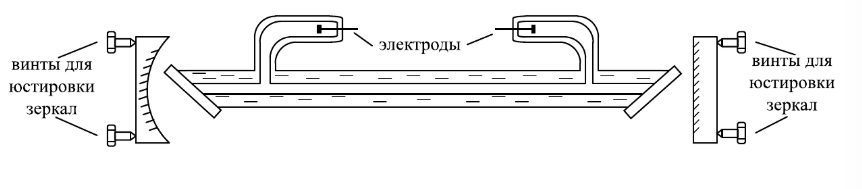
\includegraphics[width=0.7\linewidth]{img2.png}
\caption{Устройство гелий-неонового лазера}
\label{img2}
\end{figure}

Типичная конструкция гелий-неонового лазера изображена на рис.$\ref{img2}$. Обычно используется сферический или полусферический резонатор, представляющий более мягкие требования к точности юстировки зеркал и менее чувствительный к их угловым отклонениям по сравнению с плоским резонатором.

\subsection{Экспериментальная установка}

Схема экспериментальной установки приведена на рис.$\ref{img3}$. На одной оптической рельсе расположены: головка промышленного He-Ne-лазера ЛГ-75 с исследуемой газоразрядной трубкой (11), заключенной в кожух (10), рейтер с полупрозрачным зеркалом (4), фотодиоды (5 и 6), а также 3 съемных рейтера с выходным зеркалом (9), отрицательной линзой для наблюдения модовой структуры излучения исследуемого лазера или поляроидом для исследования поляризации выходного излучения лазера (8) и с белым экраном (7).

Юстировочный лазер (1) с белым экранчиком (2) и модулятор (3) закреплены на втором оптическом рельсе. Модулятор может быть повернут в разные положения: при изренеии коэффициента усиления он модулирует пучок, идущий от юстировочного лазера, при измерении поляризации излучения исследуемого лазера он модулирует выходящее из него излучение. В остальных случаях модулятор отводится в сторону, чтобы не перекрывать пучки.

Юстировочный лазер предназначен для настройки положения всех элементов установки и является источником зондирующего излучения для измерения усиления активной среды исследуемого лазера.

Зондирующий пучок сначала попадает на полупрозрачное зеркало (4). Часть излучения проходит сквозь зеркало и попадает на фотодиод №1 (6), с которого снимается сигнал, пропорциональный интенсивности зондирующего пучка. Отраженная часть направляется в исследуемую трубку.

Сигналы с обоих фотодиодов подаются на звуковую карту компьютера и с помощью PhysLab измеряются с высокой точностью. Чтобы вычислить усиление трубки по отношению сигналов с фотодиодов невозможно, используется следующий прием: вычисляется отношение сигналов с фотодиодов два раза. Один раз - при выключенном питании трубки, когда усиления нет, второй раз - при включенном питании, когда появляется усиление. Затем делится второе значение на первое и получается усиление. Для увеличении точности и удобства измерений чувствительности фотодиодов подбираются таким образом, чтобы сигналы с них были приблизительно одной величины. Для этого пучок, попадающий на фотодиод №1, ослабляется с помощью матовых пластинок, помещенных внутри кожуха фотодиода.

\begin{figure}[h]
\centering
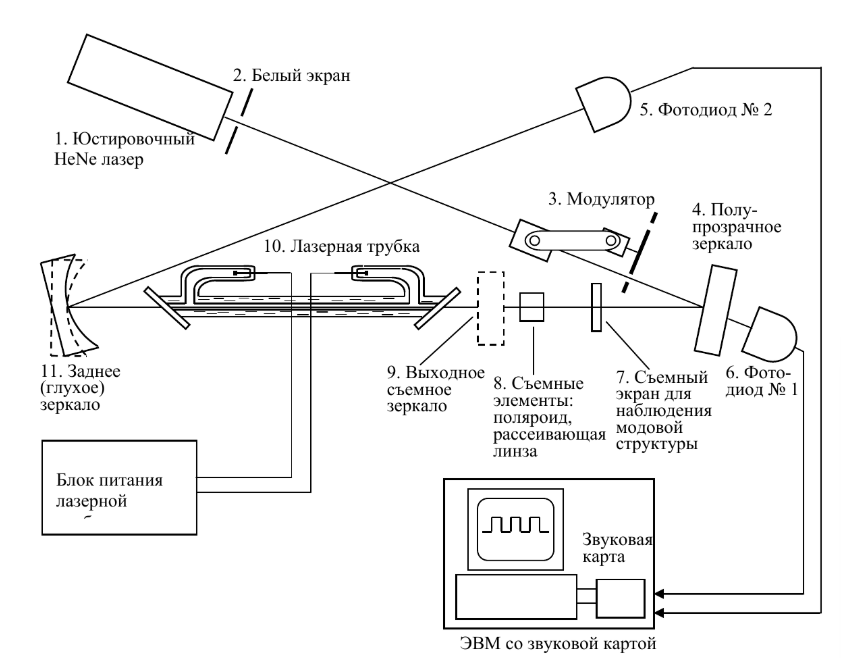
\includegraphics[width=0.7\linewidth]{img3.png}
\caption{Схема экспериментальной установки. Штриховыми линиями показано положение зеркал при получении лазерной генерации на исследуемой трубке}
\label{img3}
\end{figure}

Сигналы с фотодиодов можно измерять достаточно точным цифровым амперметром или вольтметром постоянного тока. Однако при этом нужно вычитать из показаний темновой ток фотодиода, который сильно зависит от температуры и поэтому плавает во времени, что усложняет измерения. Самый простой путь устранения влияния темнового тока - промодулировать интенсивность излучения, например, вращающимся обтюратором и перейти к измерениями на переменном токе. При этом также устраняется влияние внешних засветок и фликер-шумов, амплитуда которых растет по закону $1/f$, где $f$ - частота.

Для получения генерации вынужденного излучения лазера на исследуемой трубке используется съемное выходное зеркало (9), закрепленное в юстируемой оправе. Наблюдение модовой структуры излучения исследуемого лазера производится с помощью короткофокусной отрицательной линзы (8), позволяющей на коротком расстоянии увеличить размер вызодного пучка, и съемного белого экрана (7). Изучение поляризации исследуемого лазера производится с помощью вращающегося поляроида, устанавливаемого вместо отрицательной линзы, модулятора и фотодиода №2.

\newpage
\section{Ход работы}
\begin{enumerate}
    \item Измерим усиление трубки
    
    \begin{figure}[h]
    \centering
    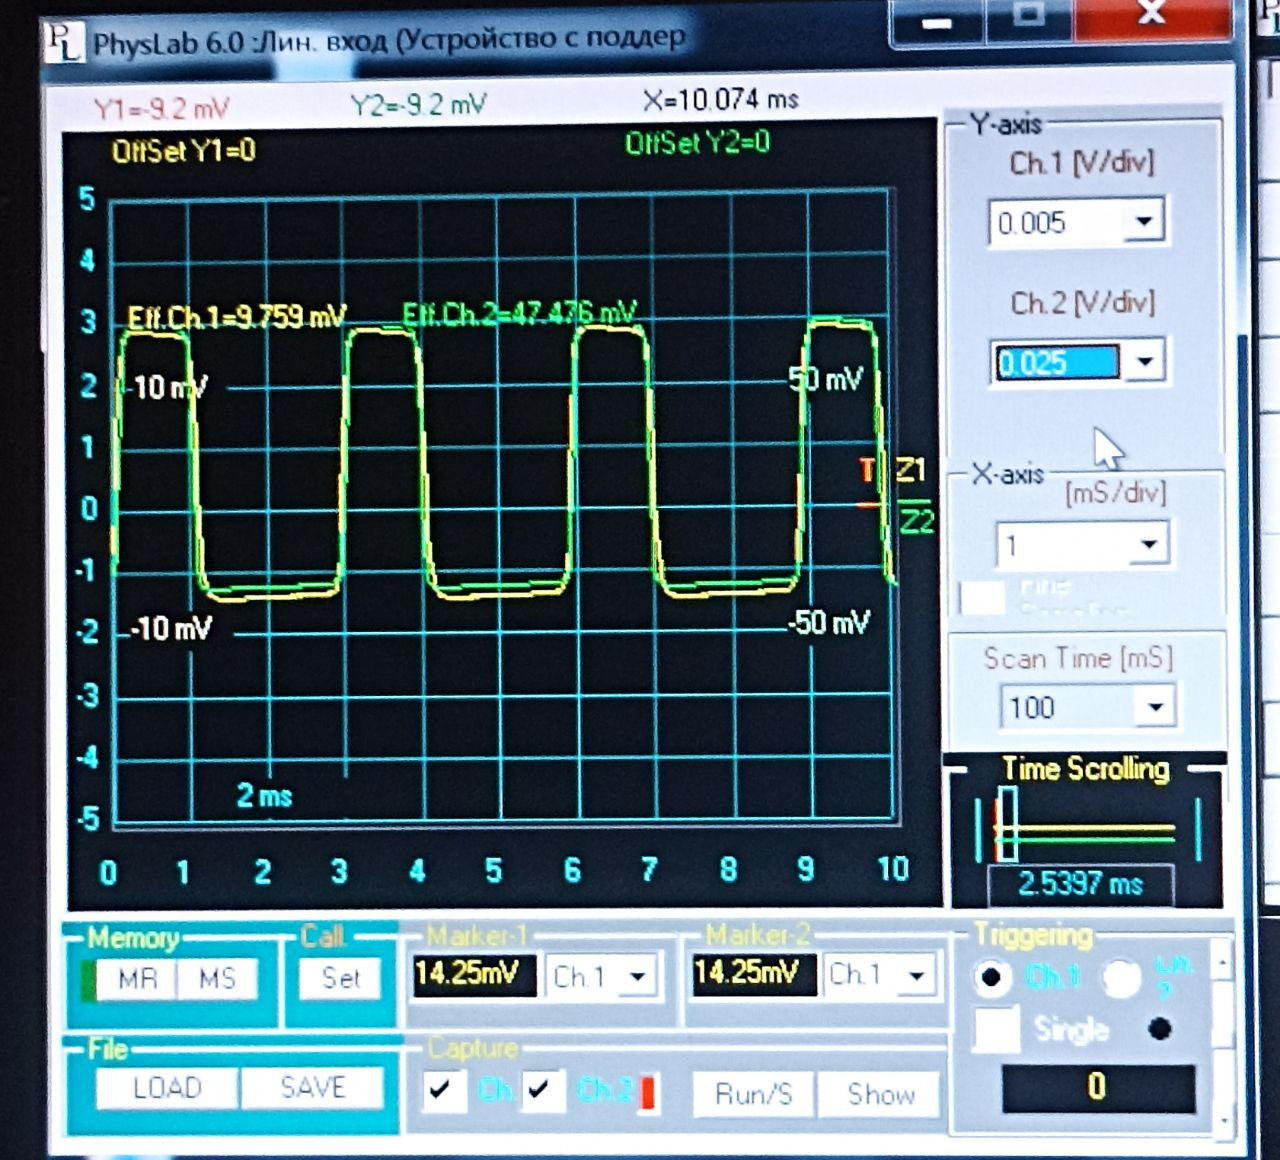
\includegraphics[width=0.7\linewidth]{photo1.jpg}
    \caption{Показания осциллографа при измерении усиления лазерной трубки}
    \label{photo1}
    \end{figure}

    Эффективное значение напряжения первого канала (с фотодиода №1):
    
    $U_\text{эф1} = (9.76\pm0.05)\text{мВ}$
    
    Эффективное значение напряжение второго канала (с фотодиода №2):
    
    $U_\text{эф2} = (47.48\pm0.05)\text{мВ}$

    Коэффициент усиления: $K = \frac{U_\text{эф2}}{U_\text{эф1}} = \frac{47.48}{9.76}=4.86$

    $\sigma_K = K\cdot\sqrt{\Big(\frac{\sigma_{U_\text{эф1}}}{U_\text{эф1}}\Big)^2+\Big(\frac{\sigma_{U_\text{эф2}}}{U_\text{эф2}}\Big)^2} = 4.86\cdot\sqrt{\Big(\frac{0.05}{9.76}\Big)^2+\Big(\frac{0.05}{47.48}\Big)^2}=0.03$

    \begin{center}
        \boxed{K=(4.86\pm0.03)(\varepsilon=0.62\%)}
    \end{center}
    
    \item Добиваемся лазерное генерации на исследуемой трубке. Исследуем состояние поляризации излучения лазера на исследуемой трубке. Измерим зависимость относительной интенсивности от угла поворота поляроида.
    \begin{table}[h!]
    \centering
    \begin{tabular}{||c||c|c|c|c|c|c|c|c|c|c|c|c|c|c||}
    \hline
        $\alpha$ & 20 & 30 & 40 & 50 & 60 & 70 & 80 & 90 & 100 & 110 & 120 & 130 & 140 & 150  \\
        \hline
        $U$, мВ & 1.0 & 2.3 & 3.7 & 6.3 & 8.1 & 6.4 & 8.6 & 11.9 & 12 & 8.8 & 7.1 & 4.3 & 3.4 & 2.0 \\
        \hline
        $\sigma_U$, мВ & 0.1 & 0.1 & 0.1 & 0.1 & 0.1 & 0.1 & 0.1 & 0.1 & 0.1 & 0.1 & 0.1 & 0.1 & 0.1 & 0.1 \\
        \hline
        $U/U_{max},\%$ & 8.3 & 19.2 & 30.8 & 52.5 & 67.5 & 53.3 & 71.7 & 99.2 & 100 & 73.3 & 59.2 & 35.8 & 28.3 & 16.7 \\
        \hline
        $\sigma_{U/U_{max}}, \%$ & 0.8 & 0.8 & 0.9 & 0.9 & 1.0 & 0.9 & 1.0 & 1.2 & 1.2 & 1.0 & 1.0 & 0.9 & 0.9 & 0.8 \\
        \hline
    \end{tabular}
    \end{table}

    Зависимость представляет собой синусоиду. Наибольшее значение интенсивности лазерного излучения достигается при $\alpha = \sim90^\circ$.

    Теоретическая зависимость для линейной полиризации:
    
    \texttt{Закон Малюса}:     
    $I = kI_0 \cos^2{\varphi} \rightarrow \frac{I}{I_0} \sim \cos^2{\varphi}$
    
    \begin{figure}[h]
    \centering
    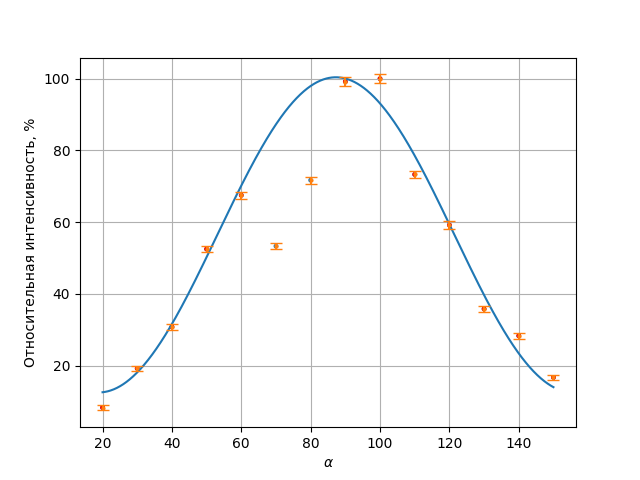
\includegraphics[width=0.9\linewidth]{graph1.png}
    \caption{Зависимость относительной интенсивности от угла поворота поляроида}
    \label{graph1}
    \end{figure}

    \item Проведем наблюдение модовой структуры лазерного излучения.

    \begin{figure}[h]
    \centering
    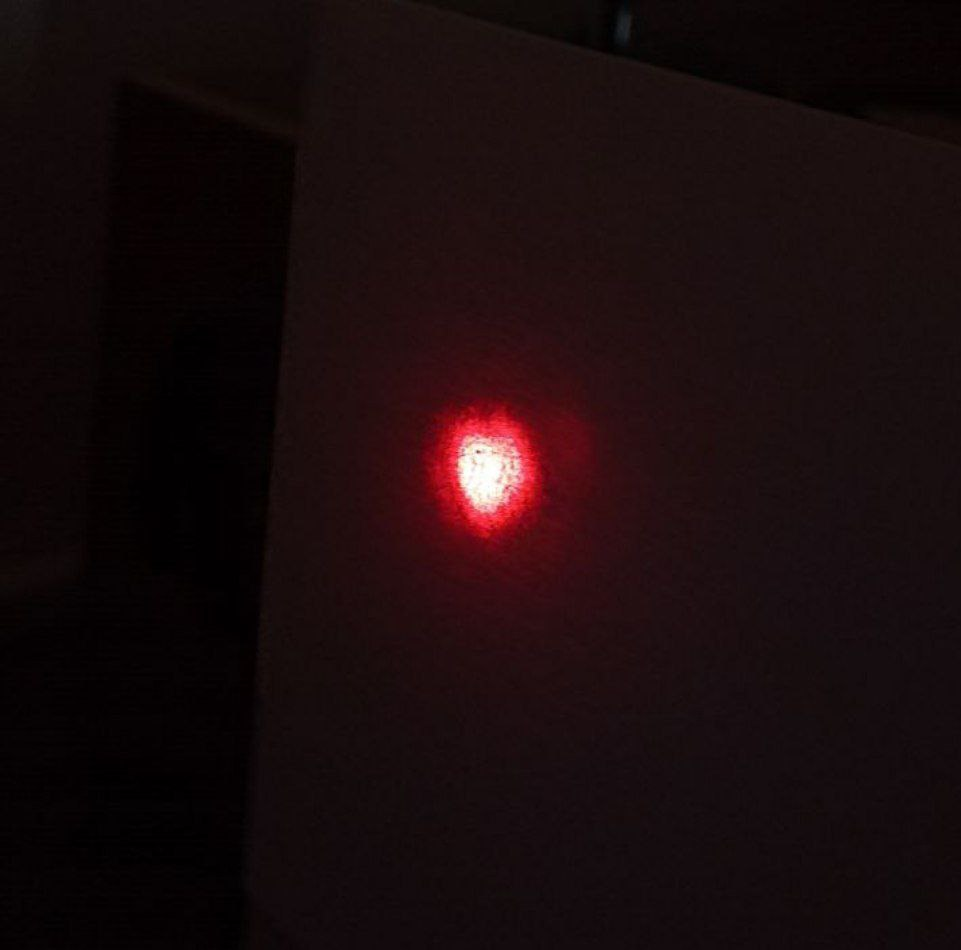
\includegraphics[width=0.4\linewidth]{photo2.jpg}
    \caption{Одномодовый режим лазера}
    \label{photo2}
    \end{figure}

    \begin{figure}[h]
    \centering
    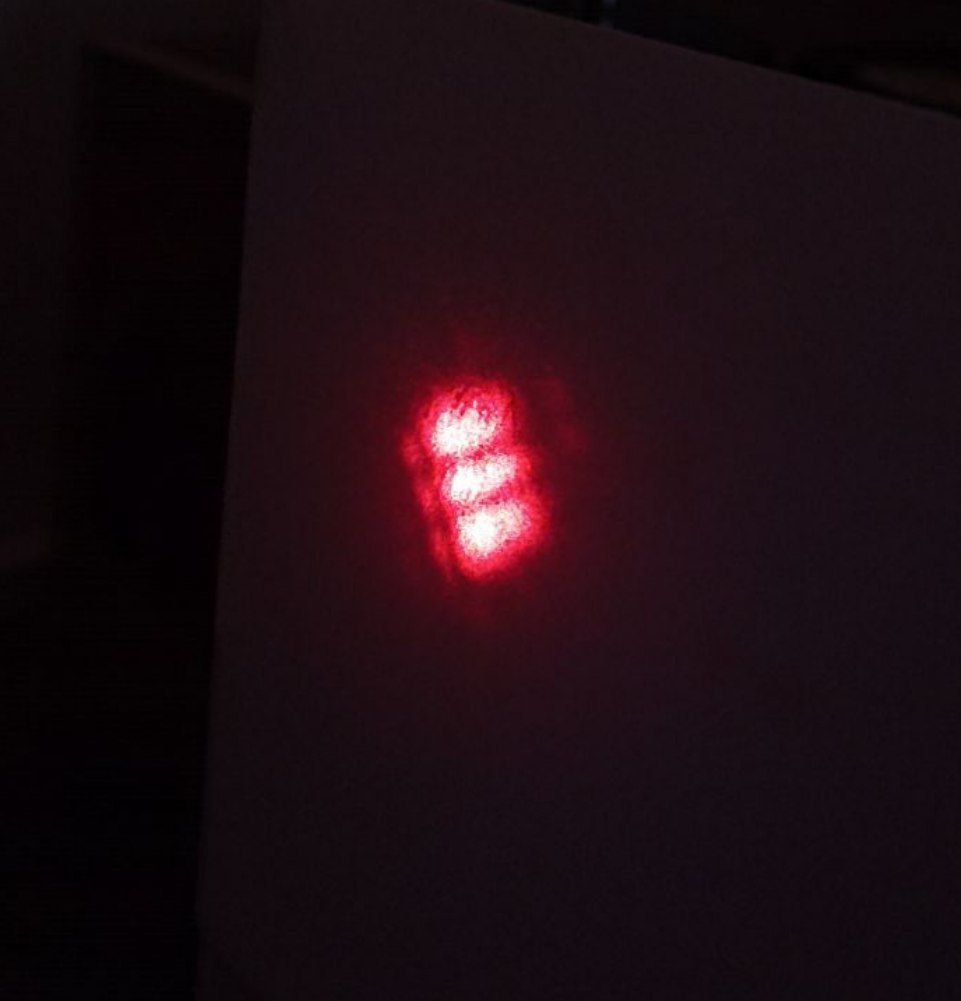
\includegraphics[width=0.4\linewidth]{photo3.jpg}
    \caption{Трехмодовый режим лазера}
    \label{photo3}
    \end{figure}

    \begin{figure}[h]
    \centering
    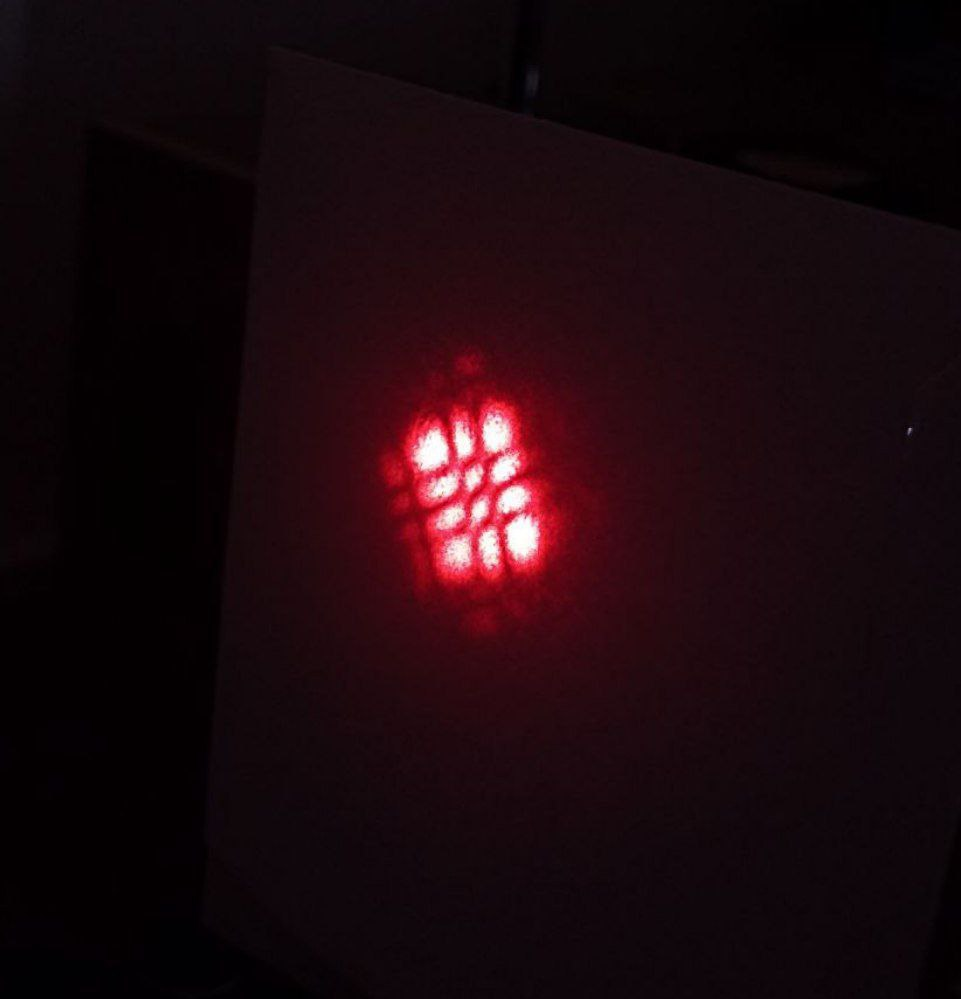
\includegraphics[width=0.4\linewidth]{photo4.jpg}
    \caption{Многомодовый режим лазера}
    \label{photo4}
    \end{figure}
\end{enumerate}

\section{Выводы}
В данной работе мы изучили основные принципы работы газового лазера и свойства лазерного излучения на примере гелий-неонового лазера. Вначале мы измерили коэффициент усиления трубки и получили невероятное значение $K = 4.86\pm0.03$. Далее мы выявили характер поляризации излучения. Зависимость оказалась синусоидальной, наибольшее значение интенсивности достигается при $\alpha\sim 90^\circ$. В конце мы наблюдали модоывй состав лазера.


Сперва мы пронаблюдали его модовый состав. Затем был выявлен характер поляризации излучения, и было выяснено, что максимум приходится на углы $38^\circ$ и $218^\circ$ поляризатора. Главным достижением работы стало исследование коэффициента усиления среды, сквозь которую проходит лазерного излучение. Значение данного коэффициента составляет $G$ = (1,033 $\pm$ 0,006). То есть за проход усиление составляет $\thickapprox 3\%$! Это достаточно немало для лабораторного лазера. Однако есть погрешности измерений, которые приводят к небольшим ошибкам и неточностям -- они составляют $\thicksim 15-20\%$. Они связаны с несовершенством техники измерения. 


\end{document}
